\chapter{Installation and maintainance}
The applications can be engaged as 2 separate ensembles, that we can call frontend and backend.
\section{Frontend}
It is an interface between application and user, in this case it is web application running on Apache server with PHP module. Also the database can run on the same server.
\section{Backend}
It is that part of application, which runs on the background and provides own records making. From the server, where backend is running, also the results distribute. If we don't have enough space, it is possible to divide the application to other server, which would take care of distribution and the records would be kept after their saving on the distributive server, e.g. by means of NFS sharing. Conversely, if we want, backend can run on the same server as frontend.

\begin{figure}[ht]
\begin{center}
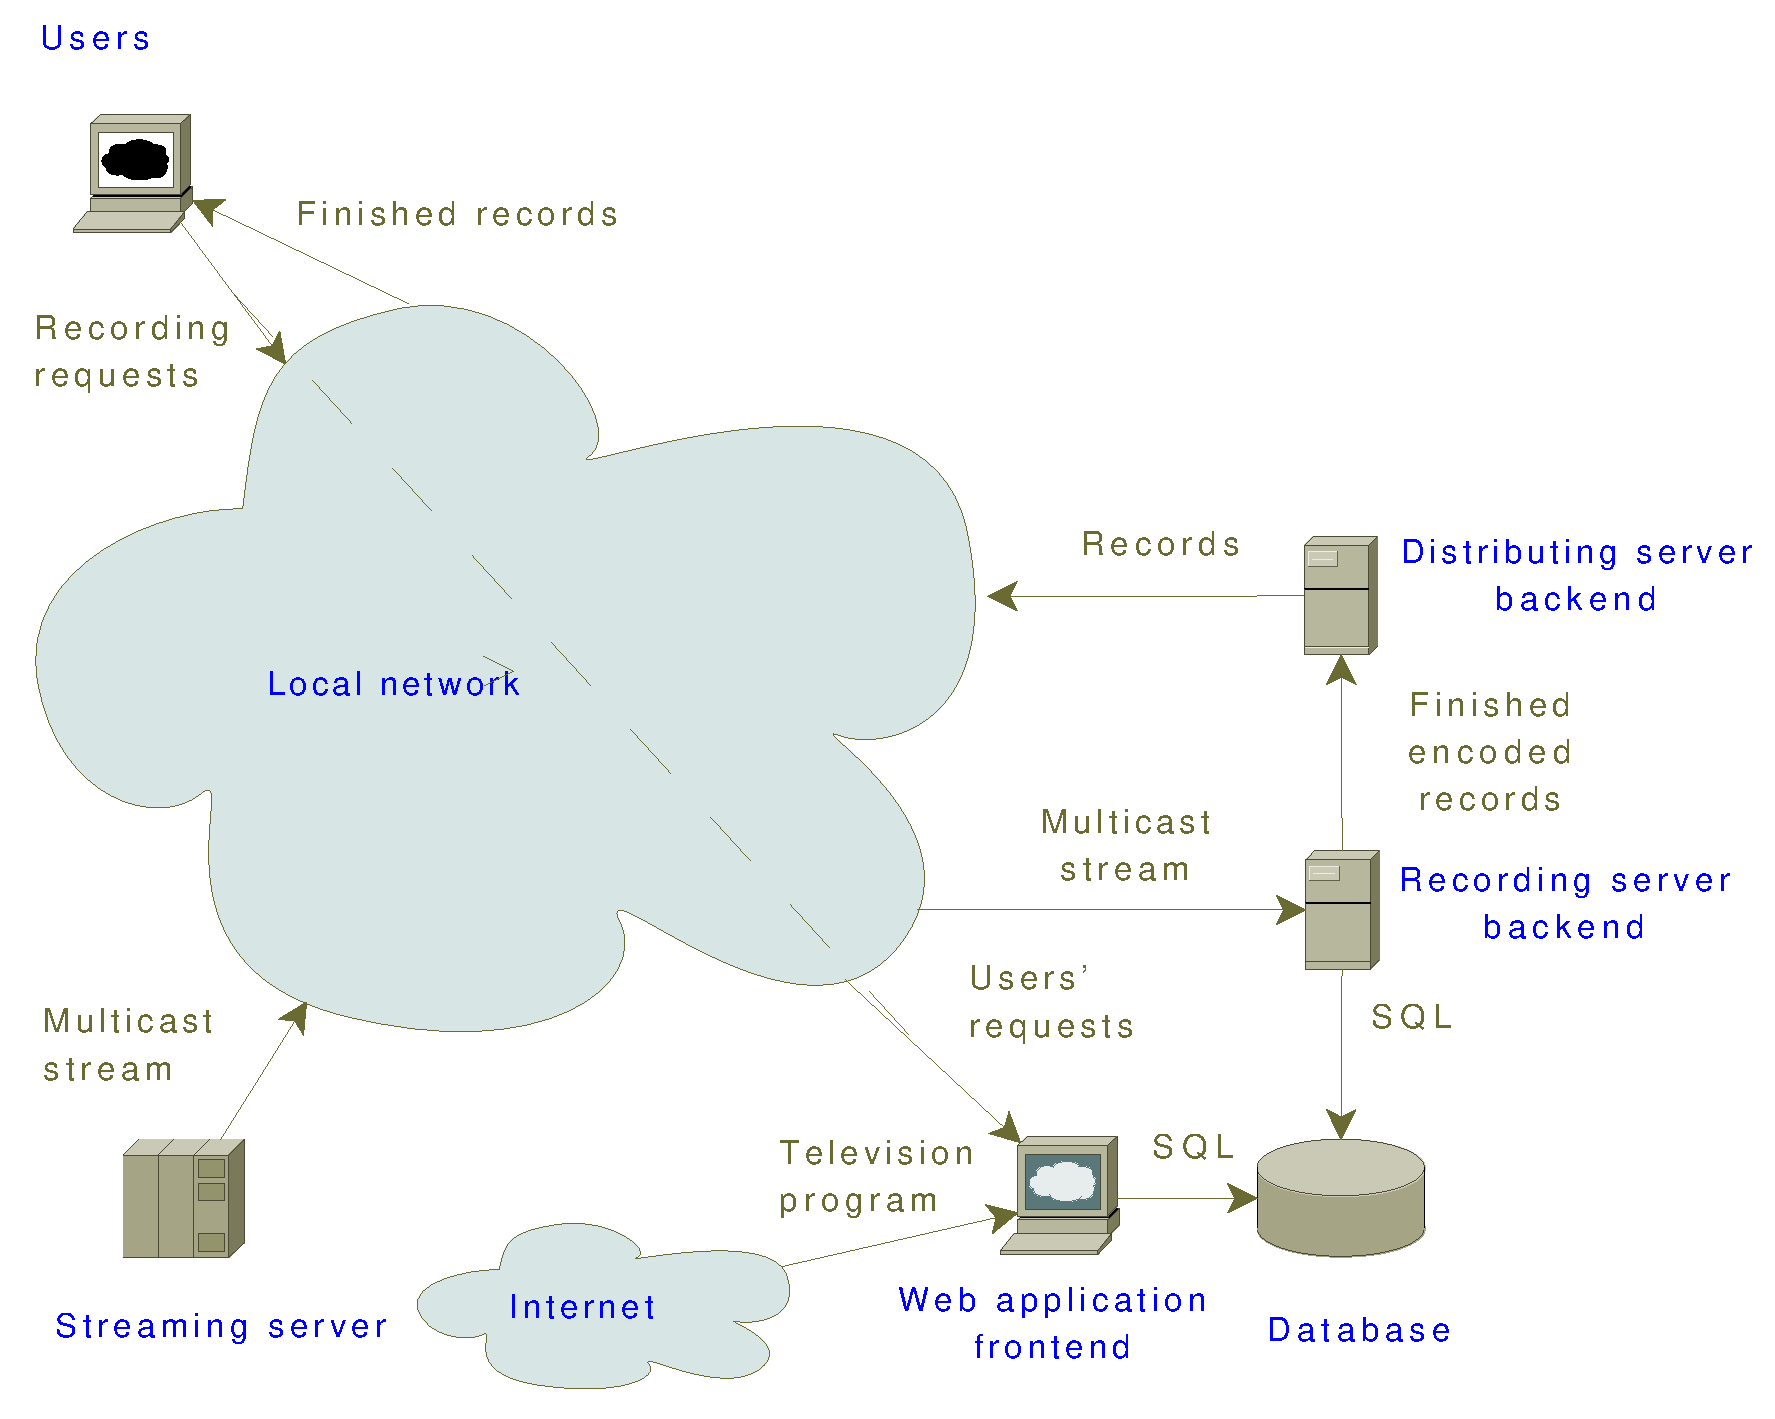
\includegraphics[width=15cm]{images/dvbgrab}
\caption{Components of DVBgrab}
\label{fig:dvbgrab}
\end{center}
\end{figure}

\section{Necessary libraries and helping programs}
\subsection{Apache}
We will need Apache as the web server both on backend and frontend server.

At least for backend server it is good to use either version 1.x or 2.2, because version 2.0 had some problems with files bigger than 2GB, what happens often to created grabs.
\subsection{PHP}
It is necessary to have module to Apache on web server. On recording server PHP interpreter accessible from command line is enough. Usually installation contains both. Application was tested for both PHP version 4 and 5. In PHP some extensions must be allowed, see below.
\subsection{php-pear-Log}
Log system, analogue log4j for Java. It is necessary for both servers and by means of it all messages are written to log files. 4 log files are used and they are in subdirectory log.
\bitem
\item\textbf{dvbgrab.log} -- general messages of system
\item\textbf{dvbgrab.log.sql} -- all SQL statements, which are executed
\item\textbf{dvbgrab.log.sys} -- all command line statements, which are executed by PHP
\item\textbf{dvbgrab.log.clean} -- logging output from maintainance script.
\eitem

Logging SQL and system commands can generate quite big logs, that's why after debug of application it should be turned off in dolib.inc.php.
\subsection{php-json}
Support for JSON (JavaScript Object Notation) to PHP. JSON is used for requests for a detail of TV show or record in the list of records. It is an alternative notation, which is returned for executing XMLHttpRequest from javascript. This extension facilitates generating JSON answers in the script, which loads a detail from database, and executing received answers on the web site.
\subsection{php-adodb}
A library for abstract approach to different databases. All executions to database translates from its syntax to syntax of used database machine.

\subsection{XMLTV}
If you want to use XMLTV module for loading television program, it is necessary to install this package. Either you'll find right there downloading script or you'll appreciate at least script tv\_sort.
\subsection{Database}
DVBgrab should work with any database, that is supported in ADOdb. It is tested on PostgreSQL and MySQL, also the scripts for founding of database are ready in syntax for MySQL and PostgreSQL.
\section{Downloading DVBgrab}
DVBgrab is accessible on sourceforge.net. Available are also both published versions and reading from development repository subversion.

You'll find a link to versions on the website of the project http://dvbgrab.sourceforge.net/.

For export from the repository subversion use this:

Older version \textbf{dvbgrab-1.0}
\begin{small}\begin{verbatim}
svn export --username anonymous \
https://dvbgrab.svn.sourceforge.net/svnroot/dvbgrab/tags/dvbgrab-1.0 dvbgrab
\end{verbatim}\end{small}
Actual version \textbf{dvbgrab-2.0}
\begin{small}\begin{verbatim}
svn export --username anonymous \
https://dvbgrab.svn.sourceforge.net/svnroot/dvbgrab/tags/dvbgrab-2.0 dvbgrab
\end{verbatim}\end{small}
\textbf{Development version}
\begin{small}\begin{verbatim}
svn export --username anonymous \
https://dvbgrab.svn.sourceforge.net/svnroot/dvbgrab/trunk dvbgrab
\end{verbatim}\end{small}

\section{Founding of database}

In the subdirectory sql there are ready scripts convert.sh, mysql.sql, postgres.sql, data.sql.
\bitem
\item\textbf{convert.sh} -- is for conversion database data from dvbgrab-1.0 to dvbgrab-2.0, though this conversion isn't recommended and it is more safe to convert only users' accounts. Both versions of DVBgrab keep running concurrently for some time (old DVBgrab keep available e.g. under another name) and actual requests let be solved in original version and when they are executed, cancel the old version and keep only the new one
\item\textbf{mysql.sql} -- founds all necessary charts for DVBgrab on MySQL
\item\textbf{postgres.sql} -- founds all necessary charts for DVBgrab on PostgreSQL
\item\textbf{data.sql} -- inserts some initial notations into the charts. 
\eitem

Into the chart param it inserts date of the last updating of users' accounts (sometimes in former times). 

Into the chart tvgrabber adds two notations of scripts for downloading television program. These notations can be further modified by means of web configuration interface, but we can modify them already here. At least it would be good to choose some random terms of starting in cron, so that all installations of DVBgrab won't connect to servers along with the program. Into the chart the encoder will add five notations, one for MPEG-2 and four for MPEG-4 with differently big resolution of notation.

Then it will add television channels (ČT1, ČT2, Nova, Prima) to channel. Now it is good to check IP addresses and ports, from which system has to save the channels and to make sure that eventual xmltv module uses the same ID of channel as in this chart. If we add new channel, we determine also new name of the file with logo and we save logo to directory images.

Finally we can add several messages for users into the chart, that will display on the web interface in section News.

\section{Configuration of DVBgrab}

We save downloaded directory on web server to selected path (e.g. /var/www/dvbgrab). On web server apache we can set virtual server, which publishes directory with DVBgrab under another URL than the name of server, e.g. http://dvbgrab.domain.cz.

As initial file we use distributional configuration file config.php.dist, which we copy as config.php.
We check, if ADOdb refers to the library php-adodb, in case of need we modify target of the reference so that it will correspond to our ADOdb (in accordance to distribution).

If we want to use web configuration interface, it is necessary to set the right of writing also for the user, under who web server runs. We can provide that by starting of script configure.sh. Now we can begin to use administrative interface, which should be available on URL http://dvbgrab.domain.cz/setup.php. Eventually we can set everything directly by editing of file config.php.

More detailed description of options of the configuration file:
\bitem
\item\textbf{db\_name} -- Determins the name of database, which we founded for DVBgrab.
\item\textbf{db\_type} -- Determins the type of database server, one of (access, ado, ado\_access, ado\_ms-sql, db2, odbc\_db2, vfp, fbsql, ibase, firebird, borland\_ibase, informix, informix72, ldap, mssql, mssqlpo, mysql, mysqlt, maxsql, oci8, oci805, oci8po, odbc, odbc\_mssql, odbc\_oracle, odbtp, odbtp\_unicode, netezza. pdo, postgres, postgres64, postgres7, postgres8, sapdb, sqlanywhere, sqlite, sqlitepo, sybase, sybase\_ase).
\item\textbf{db\_host} -- The name of computer, on which database runs.
\item\textbf{db\_user} -- The name of database user.
\item\textbf{db\_pass} -- The password for access into database.
\item\textbf{auth\_db\_used} -- Determins, if users will be allowed to use password from any other external database. It means that if we have e.g. database of users of local network and there passwords for any other services, then we can check users there.

Then the registration will check, if such user exists in external database. If he exists, he has to write the same password as the user of selected name has in external database. If he writes right password, he can be registered and in database of DVBgrab there is instead of his password only word \quotedblbase extern'', which means that user uses external password. If the password doesn't correspond to external database, the registration is refused. If user with such name doesn't exist in external database, the registration can be executed and the password is saved into database of DVBgrab. The value 1 means to use external database, the value 0 means not to use.

User with external password is also limited that he can't change password by means of DVBgrab and also new generated password can't be sent to him in case of forgetting it (that should be solved by systems above external database).
\item\textbf{auth\_db\_used\_only} -- Determins if also other users (than those with external password) can be registered and use DVBgrab. That's a way how to limit DVBgrab only for the users, who are registered in our external database (e.g. only registered users of local network). The value 1 means only those with external password, the value 0 means also the others.
\item\textbf{auth\_db\_name} -- The name of external database in database machine.
\item\textbf{auth\_db\_type} -- The type of database for external checking, it can gain the same values as db\_type.
\item\textbf{auth\_db\_host} -- The name of computer, on which database for external checking runs.
\item\textbf{auth\_db\_user} -- The name of database user with access into external database.
\item\textbf{auth\_db\_pass} -- The password of this user for access into database.
\item\textbf{auth\_db\_select} -- SQL request for checking password of user, in this string two text strings will be replaced, dvbgrab\_username is replaced by filled user's name and dvbgrab\_password is MD5 of filled password. If this select returns at least one line, user's name and password are accepted.
\item\textbf{auth\_db\_user\_select} -- SQL request for user, if he exists in external database. In this string only dvbgrab\_username will be replaced. If at least one line returns, the user exists in external database. Returned lines should have the structure user's name, password in MD5, user's e-mail, ip address. If we can't determine any columns in accordance to external database, we return in corresponding column NULL.
\item\textbf{error\_status} -- Amount of information about originated error:
\bitem
\item 0 -- Each error is published on website.
\item 1 -- Each error is sent to designated e-mail.
\item 2 -- Each error is ignored. This is default setting.
\eitem
\item\textbf{error\_email} -- E-mail, where information about errors of the web interface will be sent.
\item\textbf{admin\_email} -- E-mail, where information about errors in recording system will be sent and from this e-mail e-mails to users will be sent.
\item\textbf{report\_email} -- E-mail, where summary information about using of system will be sent.
\item\textbf{proxy\_server} -- IP address of HTTP proxy server, if it has to be used for access to external websites (for downloaders television program).
\item\textbf{proxy\_port} -- Port for HTTP proxy.
\item\textbf{grab\_history} -- How many days recorded TV shows for downloading have to be kept.
\item\textbf{tv\_days} -- For how many days in advance television program has to be loaded.
\item\textbf{midnight} -- What hour we'll consider as midnight by dividing TV shows into single days. (Then we understand a television day e.g. from six hour in the morning to six hour next day.)
\item\textbf{hour\_frac\_item} -- To how big sections we'll aggregate the list of TV shows. 24 should be dividable by the value without rest. That provides vertical alignment of all television channels.
\item\textbf{grab\_quota} -- How many records a week the user can request.
\item\textbf{user\_inactivity\_limit} -- After how many days of inactivity user's account will be removed.
\item\textbf{dvbgrab\_log} -- To which file information about recording process has to be saved.
\item\textbf{grab\_date\_start\_shift} -- How many minutes beginning of recording TV show has to be moved, contrary to planned beginning of TV show.
\item\textbf{grab\_date\_stop\_shift} -- How many minutes the end of recording TV show has to be moved, contrary to planned end of TV show.
\item\textbf{record\_time\_after\_last} -- How long to record selected TV show, if we don't know next TV show (e.g. the last TV show in the night has next one next day in the morning). We set it in seconds.
\item\textbf{hostname} -- The name of computer, from which we distribute ready records. Eventually it can be also the whole preliminary part of URL (if we don't have virtual host in apache set into user's directory). It doesn't end by slash, so e.g. \quotedblbase http://grab.domain''.
\item\textbf{grab\_storage} -- The directory, to which TV shows will be saved. It is shared directory of all users. It doesn't end by slash.
\item\textbf{grab\_storage\_size} -- How many GB space we have reserved for recorded TV shows. (Limited by the size for directory grab\_storage).
\item\textbf{grab\_storage\_min\_size} -- Minimal amount of free space on recording disc, when we start to remove older records.
\item\textbf{grab\_root} -- The directory, where references to ready TV shows will be saved. It has to be accessible for http server. In this directory users' directories will be founded. It doesn't end by slash.
\item\textbf{grab\_backend\_lang} -- The language, used in backend scripts (cz, sk, en, fr, ..). This will be used only in the case that the message is been sending to admin of DVBgrab or to user, whose last used language isn't saved yet.
\item\textbf{grab\_backend\_strip\_diacritics} -- The sign, if national characters in recorded files should be replaced by their ASCII equivalents, or if the part of the name of record is only ID number of record. Diacritics in some file systems might be not supported or not set to UTF-8, in which we have the names of TV shows. That's why removing diacritics is used, but it isn't possible to solve diacritics completely universal for all characters from UTF-8. For Czech language it works good, in Chinese it would be better to use only ID. The name of TV show including diacritics is then in associated descriptive XML file. The value 0 determins using of ID, the value 1 the name of TV show.
\eitem

In the last part there is a definition of downloaders television program. We can allow or forbid predefinated. We can also define the new one. Each downloader has 3 important parameters:

\bitem
\item\textbf{tvg\_name} -- The name of downloader.
\item\textbf{tvg\_cron\_time} -- The time of planned starting by means of cron daemon. Syntax of cron is directly set, that means 5 numbers indicating in sequence minute, hour, day in a month, month, day in a week. Instead of number we can use either asterisk (it means that this data doesn't matter) or */N, where N determins multiple unit, in which command has to be started (*/5 by minutes means each whole multiple 5 minutes). Then the value \quotedblbase 0 23 * * 6'' means that downloader has to be started every saturday, at 23:00. We choose these data preferably for night-time, when servers of provider won't be under heavy load. Also we try to choose them randomly if possible to minimalize probability that all installations of DVBgrab download from the same servers at the same time.
\item\textbf{tvg\_cron\_cmd} -- The command, which has to start cron daemon. Usually it will start with setting of working directory to downloading scripts, so that downloading scripts can load helping libraries from DVBgrab on the basis of their relative paths.
\eitem
If we are already satisfied with configuration, we use the button \quotedblbase Save''. That will update the file config.php and writes us information about actual configuration for cron daemon. There we replace \quotedblbase BACKEND\_DIR'' by real directory, from where backend scripts will be started and we'll copy the statement into the box. On recording server we'll use command crontab -e for editing configuration of cron daemon and we'll insert text from the box. Thereby we establish periodical executing of maintainance script, sending information about using DVBgrab and starting downloaders television program.

If we have recording server separately, it is necessary to move directory backend there. The best way is to do it by means of tar archiver, which replaces symbolic references from directory backend to shared files by their real copy. Then we extract created archive on target server and we replace subdirectory adodb either by right symbolic reference or we keep the copied one from the first server.

Automatic starting of DVBgrab, when the system starts, is provided by script service/dvbgrab, which we modify in accordance to actual location of script dvbgrab\_service and we copy it to directory in accordance to distribution (e.g. /etc/init.d/dvbgrab). Then we'll plan, in which runlevels the service will start and where will stop.


\section{Udržba záznamového serveru}
\section{Udržba uživatelů}

Je potřeba zajistit automatické promazávání hotových nahrávek, pokud dochází na serveru přidělený diskový prostor. A to jak vlastních záznamů, tak odkazů na ně v uživatelských adresářích, ale také označit v tabulce request, že daný odkaz již není platný.

\vspace{10pt}

Možnost rušit uživatelské účty i bez přístupu na stránky projektu (třeba emailem na definovaný administrační účet).

\vspace{10pt}


